% Drafting format: template-repo convention (article + local neurips_2026.sty,
% self-contained, standard fonts). FSE 2027 submission converts to acmart at
% submission prep. Every number here must trace to a committed results file
% (see ../CLAUDE.md); traces are given as comments at each use.
\documentclass{article}
\pdfoutput=1

\PassOptionsToPackage{numbers, compress}{natbib}
\usepackage[preprint]{neurips_2026}

\usepackage[utf8]{inputenc}
\usepackage[T1]{fontenc}
\usepackage{hyperref}
\usepackage{url}
\usepackage{booktabs}
\usepackage{amsfonts}
\usepackage{amsmath}
\usepackage{amssymb}
\usepackage{microtype}
\usepackage{graphicx}
\usepackage{float}
\usepackage{algorithm}
\usepackage{algpseudocode}

\begin{document}

\title{Who Grades the Grader? The Verification Gap in Self-Testing Code Agents}
\author{%
  Brian Sam-Bodden \\
  Integrallis Software
  \And
  Jyoti Vasudev \\
  Microsoft
  \And
  Josh Meyers \\
  Independent Researcher
  \And
  Eric Kasper \\
  Independent Researcher
}
\maketitle

\begin{abstract}
Agentic software engineering rediscovers the Test-Driven Development loop at machine speed:
an LLM writes tests from a natural-language specification, an LLM writes code against those
tests, LLM-as-a-judge reviewers gate each step, and the pipeline reports success once its
code passes its own tests. Nothing in that loop checks whether the tests mean what the
specification says. We call the resulting failure mode the \emph{verification gap}: problems
a pipeline reports as solved that fail held-out benchmark tests it never sees. On HumanEval
and a post-training-cutoff LiveCodeBench window, an instrumented TDD pipeline shows the gap
is systematic: when a single cheap model writes the tests, writes the code, and judges both,
about one reported success in four is false, always with the same signature---tests and code
that agree with each other but not with the specification. The remedy builders reach for, a
frontier model as test author or judge, buys completeness (on single-function problems), not
soundness: wrongly rejected correct solutions go to zero on unseen problems and frontier-judge feedback lifts true
success there by a third, but the false-accept count does not clear the decision
bar---not under a frontier test author or judge, and not for any of three frontier verifiers.
Replicating on RGRBench, a released corpus of $89$ application-scale
Python packages with hand-verified, error-barred oracles, the gap widens to two claimed
successes in five, grows with application complexity, worsens as the pipeline retries itself,
and is again not reduced by a frontier judge. A cheap generator coached by a frontier reviewer
is an efficient configuration at single-function scale, but ``all tests pass'' means only that the code agrees with
its own tests, so shipping decisions need one check from outside the loop. We release all
instruments, prompts, results, and analyses.
\end{abstract}

\section{Introduction}
\label{sec:intro}

In the early 2000s, Test-Driven Development (TDD)~\cite{beck2002tdd} appeared as a response to
the low quality and high defect rate of code that was only tested after being written. The idea
behind ``Test First'' development was to address some of the root causes of poor software quality.
One aim was to catch misunderstandings of requirements as early as possible, by making developers
turn those requirements into automated tests that everyone could agree on. These tests effectively
serve as a contract, a runnable specification for the system being built. Another aim was to
control the disorder that comes with system evolution by limiting the scope of changes and
additions to what is covered by a test. These tests reflect acceptance criteria, isolating
functionality into smaller, more focused units, which leads to better comprehension---a test-based
version of the Single Responsibility Principle (SRP), often summarized as ``do one thing and one
thing only''.

The mechanics of the process are captured in the Red-Green-Refactor loop. An atomic part of a
specification, usually an acceptance criterion, is chosen to create a test. This test is written
before any code exists. This is the ``Red'' phase: the test fails because the feature has not yet
been implemented. Now, the test sets a limit: only the minimum code needed to make it pass is
written, and nothing extra. Passing the test is the ``Green'' phase. For this to work as intended,
the test must focus on a small enough aspect that it remains narrowly targeted. The expected result
is that the code written to pass the test will not add unnecessary complexity to the system, keeping
the system's disorder in check and allowing for a more controlled, guided evolution of the codebase.
The last phase, ``Refactor,'' is optional and is used when the code can be improved, with the
safety net of passing tests in place.

Agent pipelines now run that loop independently, writing their own acceptance criteria. An LLM
takes a natural-language specification and turns it into a test suite, a second generation writes
code to pass those tests, LLM-as-a-judge reviewers check each step, and the pipeline declares
success when its code passes its tests. The pipeline comes with its own evidence.

But TDD can still fall victim to misunderstandings of the requirements. Those misinterpretations
are now locked into code that drives the pipeline. What is the value of passing tests if they are
checking the wrong thing? TDD practitioners already have a term for tests that mirror the code
instead of the requirement: the \emph{ugly mirror}~\cite{rudolph2008uglymirror}.

We will show that autonomous test-first pipelines create the conditions for the ugly mirror at
the stage where natural language is turned into tests. We call the resulting mismatch the
\emph{verification gap}: problems that a pipeline claims to have solved but that fail when checked
by an oracle the pipeline never sees (Sec.~\ref{sec:gap}).

This paper measures that gap by stress-testing an agentic test-first pipeline. In the control
setup, using a low-cost, non-frontier model in every role (hereafter \emph{all-weak}), the gap is
persistent and appears on both sides. Out of 30 problems per run, an average of $4.0$ reported
successes fail HumanEval's strong oracle ($18\%$ of what the pipeline claims) and $4.8$ fail the
hidden oracle of a LiveCodeBench window that post-dates the generator's training cutoff ($29\%$ of
claims), while $5.4$ and $3.4$ correct implementations per run are discarded because the pipeline's
own faulty tests rejected them.
% trace: experiments/exp006_model_asymmetry/results/ANALYSIS.md (control_rerun)
% trace: experiments/exp007_lcb_asymmetry/results/ANALYSIS.md (control)

The most common fix for a model that misunderstands a requirement is to use a stronger model
to write the tests. LLM-as-a-judge is also widely used to review the generated code at every
stage. Production systems are increasingly using this asymmetric approach: a cheap model generates,
and a frontier model is used somewhere in the verification roles. The \emph{test author} turns the
specification into a test suite, and the \emph{judge} reviews the tests and code and examines the
failures. We test these approaches as well: we place a frontier model in the test-author role, the
judge role, and both, while keeping a fixed weak generator (gpt-4o-mini) on both benchmarks. We
then repeat the design across three frontier verifiers and three providers (GPT-5.6 Terra,
Gemini-2.5-Pro, Claude-4.5-Sonnet; Sec.~\ref{sec:design}). The result is the main finding of the
paper: \textbf{the strength of verification is asymmetric}. The false-accept count (the gap itself)
does not pass the decision threshold in any configuration, on any benchmark, in any of the three
verifiers. False rejects drop to zero under the frontier judge---in every LiveCodeBench run with
GPT-5.6 Terra---and on unseen problems, its feedback improves the true success rate by five to six
problems in thirty ($p \leq .04$). It helps the weak generator write better tests and better code,
but its verdict is as limited as the weak judge's. Having a frontier model write tests does not
change the outcome at all.

\paragraph{From algorithm to application scale.} Both HumanEval and LiveCodeBench above were
designed as single-function, mostly algorithmic problems and do not represent software applications
that have stateful behavior, multiple files, classes, or components, and complex collaboration
patterns between them. To check if the gap we are measuring is just an artifact of toy problems, we
built RGRBench: $89$ Python packages that are stateful and cover multiple concerns (event sourcing,
reservations, billing) across three difficulty levels, each with a hand-verified suite that has its
own measured blind-spot rate (mutation kill rate $0.981$, every surviving mutant classified). This
set of applications was created in a TDD style by translating and curating TDD examples from other
programming languages when no Python version was available.

Our TDD pipeline was run against $89$ packages using only their extracted and curated
requirements, never showing the tests or code. We ran $534$ runs and found that the gap does not
shrink at this scale; in fact, it grows. Out of these $534$ runs, about two in five claimed
successes fail the held-out oracle ($41.5\%$, $95\%$ CI $[30.4, 53.7]$). The rate goes up with
problem complexity ($31\% \to 54\% \to 86\%$ across tiers) and increases even more when the
pipeline retries the Green phase ($35\%$ on the first attempt versus $64\%$ on multiple attempts).
Once again, the frontier judge does not affect it and removes all of the false rejects. The range
matches what is seen in the literature on SWE-bench overfitting: one in five to one in three
self-test-passing patches are wrong~\cite{ahmed2025overfitting,yu2026sweabs}, and ours is the first
measurement using oracles whose error is reported.
% trace: experiments/exp010_flagship/results/ANALYSIS.md; FINDINGS.md; calibrate_adapter.py

\paragraph{Contributions.}
(1)~A definition and measurement protocol for the verification gap in self-testing pipelines,
distinguishing false accepts from false rejects, and separating visible-adjacent from held-out
oracles (Sec.~\ref{sec:gap}).
(2)~New, instrumented measurements on two benchmarks, one with contamination control, showing that
the gap is systematic: about one in four claimed successes is incorrect, across every setup,
including all-frontier verification (Sec.~\ref{sec:results}).
(3)~Model-asymmetry experiments with three frontier verifiers from three providers
(GPT-5.6 Terra, Gemini-2.5-Pro, Claude-4.5-Sonnet), all pre-registered (with hypotheses, decision
rules, and budget set before any data), requiring each contrast to meet both a minimum
effect size and statistical significance: the \emph{soundness-invariance} finding (the
false-accept count within the decision bar under a frontier test author, judge, or both---for
every verifier, on both benchmarks) and the \emph{completeness} finding
(false rejects drop to $0$; off-distribution success rate increases by $5$--$6/30$, the only
significant effects in either experiment) (Sec.~\ref{sec:results-asym}).
(4)~A mechanism account based on the pipeline's own telemetry: the frontier judge acts more like a
coach than a gatekeeper, tripling the required test volume and improving generation quality, while
still accepting the same self-consistent failures (Sec.~\ref{sec:discussion}).
(5)~A reviewed instrument with documented prompt contracts and a defect register, as well as all
runners, raw results, analyses, pre-registrations, and a runbook; every experiment
pre-registered, with null results reported as findings.\footnote{Instruments, prompts, pre-registrations,
raw results, and analyses: \url{https://github.com/integrallis/self-grading-gap}.
RGRBench: \url{https://github.com/integrallis/rgrbench}.}
(6)~An application-scale replication on RGRBench, a released 89-package TDD corpus
with mutation-measured oracle error bars: the gap increases to about $42\%$, scales with task
complexity, gets worse under refinement, and remains unchanged for a frontier judge. An automated
adapter-fidelity calibration sets the measurement instrument's own error bound at $0.000$
(Sec.~\ref{sec:results-scale}).

\section{Background and Related Work}
\label{sec:related}

\paragraph{Weak tests overestimate, in benchmarks and pipelines alike.}
EvalPlus showed that the tests in the benchmark were the weak point in code
evaluation: by expanding HumanEval's test suites, it found a significant amount of previously
unnoticed incorrect code and changed the order of model rankings~\cite{liu2023evalplus}.
LiveCodeBench addressed the related issue of contamination by using a rolling problem collection
approach~\cite{jain2024livecodebench}. We used both tools. EvalPlus serves as a reliable
oracle, and for LiveCodeBench, we rely on a post-cutoff window as a hidden oracle. In the TDD
pipeline, when the tests are weak, this overestimation happens inside the loop, and the
pipeline's own self-assessment shows the same lack of awareness that EvalPlus found in
benchmarks. At the scale of entire repositories (that is, full software projects rather than just
single functions), this same overestimation has been seen directly: when test suites are
strengthened or held out, they reject about one in five to one in three of the patches that the
original benchmark tests would have accepted~\cite{ahmed2025overfitting,yu2026sweabs}. What we
call the verification gap is the TDD-internal, agent-native version of this phenomenon, measured
using oracles whose accuracy is estimated, not just assumed; Sec.~\ref{sec:results-scale} shows
that all three tools reach similar results.

\paragraph{The ugly mirror.}
TDD practitioners have long described the failure that happens when tests are written
after the implementation already exists: the \emph{ugly mirror}~\cite{rudolph2008uglymirror},
where a test simply reflects the code and confirms what it does, rather than what it should do,
with the tautological test as the extreme case~\cite{pereira2010ttdd}. Writing tests before the
code is the standard defense: if there is no implementation to influence it, the test can only
represent the intended specification. Our subject pipelines use this order, and yet we see
that the mirror effect still appears, just at a higher level. When a model writes tests based on its
interpretation of the specification and a similar model writes code to pass those tests, both the
tests and the code can reflect the same misunderstanding, and GREEN-phase generation then
guarantees that the code matches the tests. The pipeline then reports this internal consistency
as success, but it only shows that the tests and the code are in agreement.

\paragraph{Test-first generation with LLMs.}
Providing tests with problem statements improves generation~\cite{mathews2024tdd}; TiCoder
makes the authorship of tests more interactive---a human checks the proposed tests before the
code is accepted~\cite{fakhoury2024ticoder}; TENET and TDFlow extend test-driven loops to
repository-scale agents~\cite{sun2025tenet,tdflow2025}. Testing is provided, verified by humans,
or evaluated end-to-end by the impact on pass rates. Our subject class is the fully autonomous
case, in which the pipeline authors both tests and code. What we are interested in is the
reliability of the pipeline's own verdict on itself. The benchmark oracle is outside the loop,
so the end-to-end view cannot see that.

\paragraph{Self-generated tests as a signal.}
CodeT uses generated tests to rank candidate solutions, using the agreement between test
generation and execution as an indicator of correctness~\cite{chen2023codet}. On the other hand,
ConVerTest tries ground-truth-free test creation by building consensus and using
cross-validation~\cite{convertest2026}. Both methods rely on agreement to show correctness. The
verification gap reveals the weakness in this assumption: the agreement between self-authored
tests and code is exactly what our gap set fails on for every one of its members. Our asymmetry
experiments suggest that this agreement remains incorrect even if a frontier model provides
either the tests or the code.

\paragraph{LLM judges on code.}
Benchmarks evaluating LLMs as judges for coding tasks show that these judges are only
slightly aligned with execution results~\cite{jiang2025codejudgebench}, and that LLMs
consistently struggle when checking code against natural-language
specifications~\cite{verifyfailures2025}. In our subject pipeline, we include judges as
checkpoints in the process, along with an execution gate that can override the judge's
predictions. The asymmetry experiments extend these findings: upgrading the judge to a frontier
model makes it much more useful as a \emph{feedback} tool, but does not lead to better
\emph{verdicts} from the judge itself.

\paragraph{Multi-agent code generation.}
Multi-agent SDLC frameworks have been effective at handling end-to-end
tasks~\cite{hong2024metagpt}. However, as far as we know, these frameworks do not examine their
internal quality gates beyond simply reporting pass rates after ablation. Our protocol offers a
complementary and transferable approach: any pipeline with a harness that records its executed
self-verdict and outputs can use the same measurement.

\section{The Verification Gap}
\label{sec:gap}

% Every number in this section traces to a committed result file; the trace is given in a
% comment at each use. Files live under experiments/ in the artifact repository.

\subsection{Definitions}

Consider a code-generation pipeline that, for a problem $i$ with natural-language
specification $\mathit{spec}_i$, produces an implementation $y_i$, a test suite $T_i$ that the
pipeline itself wrote from $\mathit{spec}_i$, and a self-verdict
$s_i \in \{0,1\}$, the pipeline's own claim that the problem is solved, based on running
$T_i$ against $y_i$ and from any internal quality gates (in our subject pipeline, LLM judges).
An \emph{oracle verdict} $o_i \in \{0,1\}$ is the outcome of a test suite the pipeline never
sees. We use three oracles of increasing distance from the pipeline's inputs: the
\emph{visible-adjacent oracle} $o^{\mathrm{base}}_i$ (HumanEval's original tests, which
overlap the worked examples visible in $\mathit{spec}_i$), a \emph{strong oracle}
$o^{\mathrm{plus}}_i$ (HumanEval\texttt{+}~\cite{liu2023evalplus}, whose tests go far beyond
the visible examples, by roughly two orders of magnitude), and a \emph{hidden oracle}
(LiveCodeBench's private test sets~\cite{jain2024livecodebench}, never distributed with the
problem statement at all).

The \emph{verification gap} of a run over problems $P$ is the set
$G = \{\, i \in P : s_i = 1 \wedge o_i = 0 \,\}$: problems the pipeline believes it solved and
the oracle rejects, the \emph{false accepts}. We report it as a per-run count over $|P|$ and,
where the denominator matters, as the \emph{conditional gap} $|G| / |\{ i : s_i = 1 \}|$, the
probability that a claimed success is wrong. The complementary error set
$R = \{\, i : s_i = 0 \wedge o_i = 1 \,\}$ (\emph{false rejects}: correct code vetoed by the
pipeline's own tests) completes the picture; self-verification error runs in both directions
(Table~\ref{tab:confusion}).

\begin{table}[H]
\centering
\small
\caption{Self-verification as a $2\times2$ confusion matrix: the pipeline's self-verdict $s_i$
against the held-out oracle $o_i$. The loop observes only the rows---its own verdict; the columns
are hidden from it. Both off-diagonal cells are errors, but they differ in visibility: a
\emph{false reject} fails the pipeline's own tests and can be re-examined, whereas a
\emph{false accept} passes them and is, from inside the loop, indistinguishable from a true
success. The verification gap $G$ is the upper-right cell (what \emph{soundness} concerns); the
false rejects $R$ are the lower-left (what \emph{completeness} concerns).}
\label{tab:confusion}
\begin{tabular}{lcc}
\toprule
 & oracle pass ($o_i{=}1$) & oracle fail ($o_i{=}0$) \\
\midrule
self-verdict accept ($s_i{=}1$) & true accept & \textbf{false accept} ($G$) \\
self-verdict reject ($s_i{=}0$) & \textbf{false reject} ($R$) & true reject \\
\bottomrule
\end{tabular}
\end{table}

Every element of $G$ is, by construction, a case of \emph{self-consistent misalignment}: $y_i$
satisfies $T_i$, and both together deviate from $\mathit{spec}_i$. The gap is therefore not a
measure of weak code generation, since those failures are caught internally. It measures the
pipeline's inability to notice a particular class of its own errors, the ones its self-authored
tests carry forward. In the language of TDD practice, every gap member is an ugly
mirror~\cite{rudolph2008uglymirror} the pipeline made for itself: the tests reflect an
interpretation rather than the specification, and the implementation faithfully mirrors the
tests.

\begin{figure}[b]
\centering
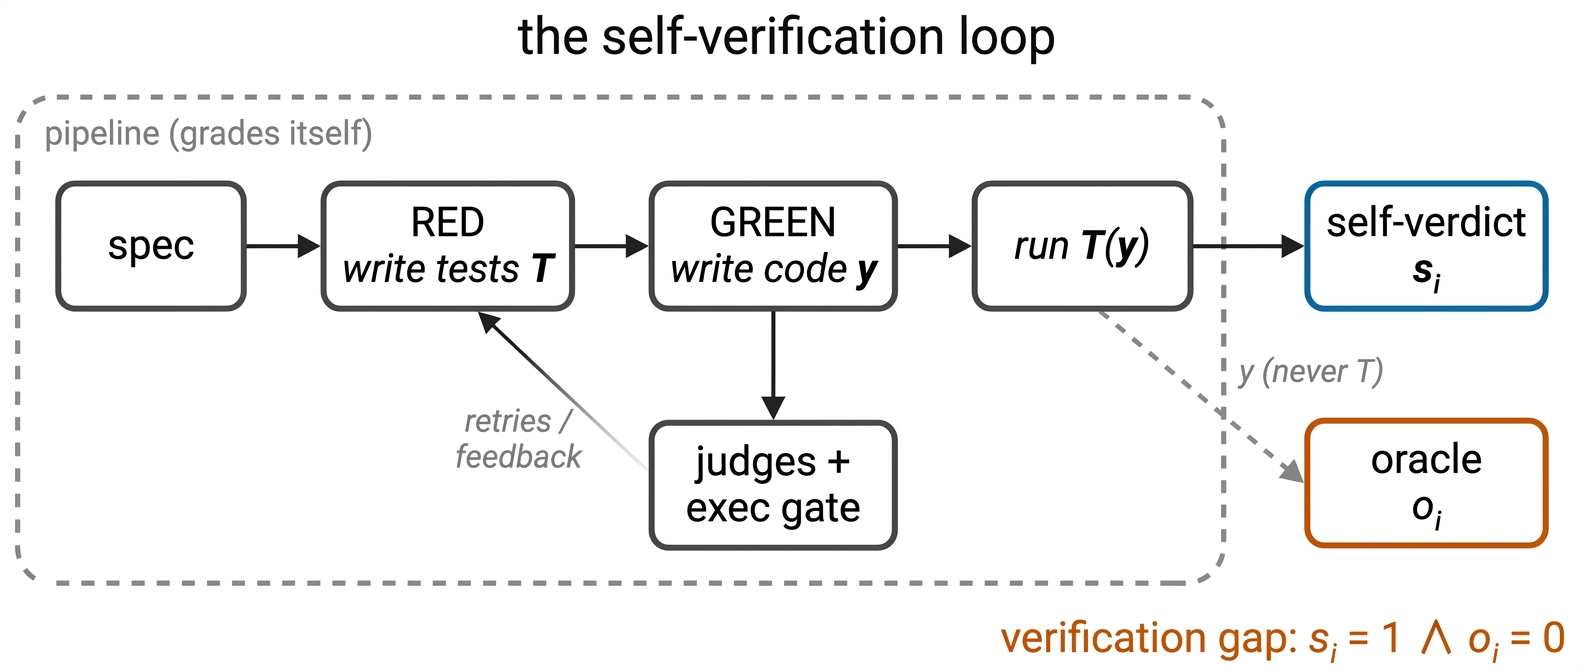
\includegraphics[width=0.9\linewidth]{figures/fig1_loop.png}
\caption{The pipeline authors tests $T$ and code $y$, grades
itself by running $T(y)$, and emits self-verdict $s_i$; the oracle sees $y$ but never $T$.
The verification gap is the set of problems where the two verdicts disagree in the pipeline's
favor.}
\label{fig:loop}
\end{figure}

\subsection{Subject pipeline}

Our subject is a test-first multi-agent pipeline in which an LLM writes tests from the
specification (RED), an LLM judge scores the tests, a second generation step writes an
implementation against those tests (GREEN), a judge predicts test outcomes, an execution
gate then runs the tests and overrides optimistic judge predictions, and a final VERIFY phase
runs the full suite, with bounded retries and textual feedback loops
(Algorithm~\ref{alg:tdd}, Fig.~\ref{fig:loop}). The pipeline's main configuration also
\emph{anchors} self-authored tests: prompt and judge together require that every worked example
in the specification appear as a test case exactly as given. Note what the execution gate cannot do:
it checks $y$ against $T$, so a wrong $T$ passes it incorrectly.

The complete instrument (engine, prompt templates, and the defect register from a
line-by-line review of the pipeline) is included with the artifact.
% trace: src/vgap/pipeline/REVIEW.md (H-1..H-15, B-1..B-10, E-1)

\begin{algorithm}[t]
\caption{Execution-gated TDD cycle (subject pipeline; generator $G$ and judge $J$ are
role-assigned per experimental cell)}
\label{alg:tdd}
\begin{algorithmic}[1]
\Require spec, test author $G_T$, code generator $G$, judge $J$, threshold $\tau$, retries $R$
\For{$r \gets 1 \ldots R$} \Comment{RED: author the tests}
  \State $T \gets G_T.\mathrm{tests}(\mathrm{spec}, f)$;\quad $q \gets J.\mathrm{score}(T, \mathrm{spec})$;\quad $f \gets J.\mathrm{feedback}$
  \If{$q \geq \tau$} \textbf{break} \EndIf
\EndFor
\If{$q < \tau$} \Return $s{=}0$ \EndIf
\For{$r \gets 1 \ldots R$} \Comment{GREEN: code against own tests}
  \State $y \gets G.\mathrm{code}(\mathrm{spec}, T, f)$;\quad $\hat{q} \gets J.\mathrm{predict}(y, T)$
  \If{$\hat{q} \geq \tau$}
    \If{$\mathrm{run}(T, y).\mathrm{allPass}$} \textbf{break} \Comment{execution gate: judge overruled by pytest}
    \Else\ $f \gets \mathrm{debugAnalysis}(T, y)$ \EndIf
  \Else\ $f \gets J.\mathrm{feedback}$ \EndIf
\EndFor
\For{$r \gets 1 \ldots R$} \Comment{VERIFY: full suite; failures route back to GREEN}
  \If{$\mathrm{run}(T, y).\mathrm{allPass}$} \Return $s{=}1,\, y,\, T$ \EndIf
  \State $f \gets J.\mathrm{analyzeFailures}(T, y)$;\quad regenerate $y$ as in GREEN
\EndFor
\State \Return $s{=}0,\, y,\, T$
\end{algorithmic}
\end{algorithm}

\subsection{Prompt architecture}
\label{sec:prompts}

Four prompts drive the loop; their structure is part of the instrument and matters to the
results, so we describe it. (Skeletons in Appendix~\ref{app:prompts}; the templates come with
the artifact under a SHA-256 manifest, with render-contract tests asserting the properties
below.)

\emph{RED generator.} Role framing (``your tests are the only specification the implementer
will see''), task description and full specification, scenario list, and finally an
\emph{anchoring block}: for every worked example in the specification, a test named
\texttt{test\_canonical\_example\_N} with the example's exact inputs and outputs and a one-line
derivation comment. There are five rules that must be followed: only test the specified behavior,
use exact signatures, compute expected values, import from the solution package, and use
plain pytest. On retries, the judge's directives and the previous attempt are included. The output
contract is a single fenced Python block.

\emph{RED judge.} The judge considers a single question: does the suite faithfully verify the
specification? This is done through a series of ordered checks: canonical-example coverage (an
anchoring block that mirrors the generator's; any missing or changed example results in the
minimum score), assertion fidelity (recalculate each expected value), no invented constraints,
coverage of all stated behaviors, and sanity. A deduction schedule links findings to a score; the
response always ends with the line \texttt{Final score: <x.xx>}, and feedback is given as
apply-verbatim \texttt{ADD:}/\texttt{REMOVE:}/\texttt{FIX:} directives, which is the feedback
channel shown in Sec.~\ref{sec:discussion} as performing the work.

\emph{GREEN generator.} The tests are given as the acceptance criterion; the rules prohibit
hardcoding test inputs and inventing behavior; the output is a single JSON object containing the
implementation file (with path, action, and content). This is the only structured output where
code appears as an escaped string field.

\emph{GREEN judge.} Predicts per-test PASS/FAIL by tracing the implementation against each
test, flags test-gaming in one line and must end with \texttt{Rating: <x.xx>} (predicted pass
fraction). The execution gate then runs the tests regardless, so this judge's optimism is limited
by pytest.

The anchoring blocks in the RED pair are delimited by markers in the template source, and the
ablation variants of the artifact (generator only, judge-side only, neither) are produced by
stripping those blocks automatically; the variant used in every run is checked on the rendered prompt
at smoke time. A fifth template, the failure analyst of the retry loops in Sec.~\ref{sec:gap},
is triggered when an execution gate or VERIFY run fails. It follows each failed test and identifies the
root cause and emits \texttt{FIX DIRECTIVES:} lines that the next GREEN attempt uses
verbatim; it presents analysis only, never code.
% trace: src/vgap/pipeline/templates/ (MANIFEST.sha256); scripts/make_variants.py;
% trace: src/vgap/pipeline/test_render_smoke.py (contract assertions)

\subsection{Measurement protocol}
\label{sec:protocol}

Three requirements make the gap measurable rather than anecdotal (Algorithm~\ref{alg:audit}).

\begin{algorithm}[t]
\caption{Verification-gap measurement over instrumented runs}
\label{alg:audit}
\begin{algorithmic}[1]
\Require pipeline $P$, problems $\mathcal{P}$, held-out oracle suites $O$, runs $N$
\For{each problem $i \in \mathcal{P}$, run $r \in 1..N$}
  \State $(y_{ir}, T_{ir}, s_{ir}) \gets P(i)$ \Comment{harness captures artifacts + the executed self-verdict}
  \State $o_{ir} \gets \mathrm{Exec}(O_i \text{ on } y_{ir})$ \Comment{standard harness (EvalPlus / LCB / RGRBench adapter), outside the loop}
\EndFor
\State $G \gets \{ (i,r) : s_{ir}{=}1 \wedge o_{ir}{=}0 \}$;\quad $R \gets \{ (i,r) : s_{ir}{=}0 \wedge o_{ir}{=}1 \}$
\State \Return $G, R$, per-run provenance and cost
\end{algorithmic}
\end{algorithm}

\emph{(1) Both verdicts measured but never reported.} The self-verdict $s_{ir}$ is an outcome
that the harness sees and not a claim the pipeline makes about itself. It is the executed result
of the pipeline's own final test run, recorded with per-call token and cost accounting. The
oracle verdict is obtained on the produced implementation outside the loop by the benchmark's own
harness: EvalPlus~\cite{liu2023evalplus}, LiveCodeBench's evaluator~\cite{jain2024livecodebench}
for the hidden-test problems, and RGRBench's hand-verified suites through a non-cheating adapter
(Sec.~\ref{sec:results-scale}). Every number in this paper comes from these two recorded
streams, the self-verdict and the oracle, and can be rebuilt from committed per-run artifacts.
% trace: src/vgap/pipeline/humaneval_runner.py, lcb_runner_local.py;
% trace: experiments/exp007_lcb_asymmetry/score_lcb.py (harness-side scoring)

\emph{(2) Oracles beyond the visible examples.} Anchoring ties $T_i$ to the
specification's worked examples, which HumanEval's base oracle partially shares; a gap
measured only against $o^{\mathrm{base}}$ understates the phenomenon. On the all-weak
setup, false accepts average $3.0$ per 30-problem run against the base oracle and
$4.0$ against HumanEval\texttt{+}.
% trace: exp006 ANALYSIS.md (control_rerun fa_base/fa_plus)
The LiveCodeBench experiment removes visibility entirely: prompts include the statement and its
public examples, while scoring uses the private suites, on problems whose contest dates
are more than a year after the weak model's training cutoff.

\emph{(3) Pre-registered noise floors.} Per-problem outcomes are unstable across
byte-identical runs: the all-weak setup disagrees with itself on $6/30$ problems (HumanEval
subset) and $9/30$ (LiveCodeBench) across five runs, with maximum pairwise pass-total
differences of $4$ and $3$.
% trace: exp006 scores/ per-run eval results; exp007 scores/ (flip counts derived in
% scripts/make_figures.py inputs; totals in each ANALYSIS.md)
Both experiments therefore fixed minimum effect sizes in advance ($4$ problems on
success-rate contrasts, $2$ on false accepts, $2$ on false rejects, $3$ on total verdict
error) that any contrast must exceed on top of statistical significance; the observed
control spreads fall at or inside these thresholds. Single-run comparisons, common in the
literature, cannot distinguish intervention effects of this size from run-to-run noise.

\section{Study Design}
\label{sec:design}

The study asks four questions.
\begin{description}
\item[\textbf{RQ1 (phenomenon).}] How large is the verification gap, against visible-adjacent,
strong, and hidden oracles, and how does it break down into false accepts and false rejects?
\item[\textbf{RQ2 (asymmetry).}] Does a frontier model in the verification roles (as test author,
as LLM-as-a-judge reviewer, or both) close the gap?
\item[\textbf{RQ3 (mechanism).}] When a stronger verifier does help, does the improvement come
from its \emph{verdicts} (better gatekeeping) or from its \emph{feedback} (better generation)?
\item[\textbf{RQ4 (scale).}] Do the size of the gap and its resistance to verifier strength persist
when moving from single-function algorithms to larger, application-scale programs that involve
multiple concerns, and how does this gap change with increasing task complexity or as the loop
itself is refined?
\end{description}

\paragraph{Experiments.} The model experiments use a single asymmetry design with four conditions
(\emph{cells}): a weak model W (\texttt{gpt-4o-mini}) generates code in every cell; a frontier
verifier S replaces W in the test-author role, the judge role (covering all three judge duties), or
both; the control condition uses W in every role. We assign the S role to three verifiers from
three different providers---GPT-5.6 Terra, Gemini-2.5-Pro, and Claude-4.5-Sonnet\footnote{\texttt{gpt-4o-mini} is
OpenAI's GPT-4o mini. The verifiers are OpenAI's \texttt{gpt-5.6-terra} (the mid-tier GPT-5.6 model,
released 2026-07-09; model card
\url{https://developers.openai.com/api/docs/models/gpt-5.6-terra}), Google's \texttt{gemini-2.5-pro}
(via Vertex AI), and Anthropic's \texttt{claude-sonnet-4-5}. All models are called through a LiteLLM
shim.}---and run this design on both benchmarks for each verifier. $N{=}5$ runs per cell, $30$
problems per run, escalation is off, and judge threshold and retries are kept the same across all
cells. Every experiment was \emph{pre-registered}: hypotheses, decision rules, and budget limits
were all committed to the repository before any API calls, so the analyses test predictions rather
than fit to the data. The primary pair uses GPT-5.6 Terra: exp006 runs a HumanEval subset that
includes previously unstable problems, scored by both EvalPlus oracles, and exp007 repeats this
on contamination-controlled data---all $19$ easy plus the first $11$ medium LeetCode problems from
LiveCodeBench release~v6 with contest dates $\geq$~2025-01-01, chosen by a deterministic rule fixed
in advance after a pilot identified the weak model's measurable range, and scored by the private LCB
suites. The FR reduction and FA invariance seen in exp006 were registered as confirmatory
predictions for exp007 before its first API call. A pre-registered replication (exp011) then reruns
both benchmark designs with the two non-OpenAI verifiers, Gemini-2.5-Pro and Claude-4.5-Sonnet, to
test whether the soundness null depends on which frontier model is used (Sec.~\ref{sec:results-asym}).
% trace: experiments/exp006_model_asymmetry/README.md, exp007_lcb_asymmetry/README.md,
% exp011_verifier_generalization/PRE_REGISTRATION.md (pre-registrations);
% experiments/pilots/README.md (band-location pilot)

\paragraph{The application-scale experiment.} A third experiment (exp010) moves to
RGRBench's $89$ packages. The pipeline receives only each package's requirements document
(user-story acceptance criteria derived solely from the tests, with the tests themselves never
shown) and is graded by the hidden, hand-verified suite through a non-cheating adapter
(Sec.~\ref{sec:results-scale}). The design keeps the soundness-invariance contrast in its most
significant form: a \emph{control} cell (weak model in every role) versus a \emph{strong-judge}
cell (GPT-5.6 Terra in all judge duties), with $N{=}3$ runs per package per cell ($534$ runs). Since
RGRBench labels each package by difficulty tier and the harness records whether a claim was made on
the first try or only after retries, these same runs test whether the gap increases with complexity
(H-D4) and whether refinement makes it worse (H-D2), both pre-registered before the first call.
% trace: experiments/exp010_flagship/README.md (pre-registration); results/plan.json

\paragraph{Statistical protocol.} All comparisons are paired by problem. For a contrast between
cells, we take each problem's majority outcome over the five runs and use the exact McNemar test on
the discordant pairs; we also require the mean per-run difference to be greater than the minimum
effect sizes from Sec.~\ref{sec:protocol}. We refer to this pair of requirements (minimum effect
size \emph{and} $p<.05$) as the \emph{decision bar}; any difference that meets only one of the two
is reported as within noise. Results for cells are reported as per-run totals, not as single runs.
Null results are reported as results.

\paragraph{Telemetry.} Every LLM call is logged with token counts, cost, and a problem, cell,
or run tag. This telemetry enables the mechanism analysis described in
Sec.~\ref{sec:results-mech}, and it is included with the artifact. Table~\ref{tab:config} lists the
configuration that remains fixed across all cells.
% trace: per-run usage.jsonl files; totals in each asym_summary.json

\begin{table}[t]
\centering
\small
\caption{Pipeline configuration held fixed across all cells.
The frontier model is called at its provider-default temperature; \texttt{max\_tokens},
\texttt{top\_p}, and seed are left unset (provider defaults).}
\label{tab:config}
\begin{tabular}{ll}
\toprule
Setting & Value \\
\midrule
Code-generation temperature & $0.7$ \\
Test-generation temperature & $0.7$ (weak author) / $1.0$ (frontier author) \\
Judge temperature & $1.0$ \\
Judge acceptance threshold $\tau$ & $0.70$ \\
Retries $R$ (RED and GREEN) & $3$ \\
Test-execution timeout & $30$\,s \\
Oracle-execution timeout & $120$\,s \\
\bottomrule
\end{tabular}
\end{table}

\paragraph{Threats addressed by design.} HumanEval is the field's best-known benchmark and
predates the training data of all current models, so we consider it within-distribution. The
LiveCodeBench window serves as the off-distribution check, since its problems were released more
than a year after the weak model's training data. No benchmark identifier is ever shown to any
model: we checked all $7{,}962$ logged prompts from both experiments and confirmed that rendered
prompts include only the problem statement and its worked examples, never a problem number or
benchmark name that a memorizing model might recognize. The training cutoff for the frontier model
is not public; Sec.~\ref{sec:threats} explains why the design remains robust in the relevant
direction. Both problem sets are selected for measurability (with increased hardness; within the
weak-model band), so per-run counts do not represent benchmark rates and are never reported as
such.

\section{Results}
\label{sec:results}

\subsection{RQ1: the gap on the corrected instrument}
\label{sec:results-gap}

Table~\ref{tab:cells} presents the full result matrix; Figure~\ref{fig:asym} shows the
error breakdown. On the all-weak control, the gap appears on both benchmarks and both sides.
For each 30-problem run, HumanEval: $24.0$ oracle passes, $4.0$ false accepts compared to
the strong oracle ($18\%$ of reported successes), $5.4$ false rejects. LiveCodeBench (hidden
oracle, post-cutoff problems): $15.2$ oracle passes, $4.8$ false accepts ($29\%$ of claims),
$3.4$ false rejects. Contamination does not account for the LCB gap: the weak model has never
encountered these problems, and the private tests are never included in any prompt. Every false
accept is, by design, a self-consistent misalignment, with tests and code agreeing with each
other but not with the specification. Every false reject is correct code that the pipeline paid
to generate but then discarded due to its own tests' veto.
% trace: exp006 ANALYSIS.md control_rerun; exp007 ANALYSIS.md control

\begin{table}[t]
\centering
\caption{Complete result matrix: per-run means over $N{=}5$ runs of 30 problems (per-run
values in the committed analyses). FA = false accepts (HumanEval: strong oracle; LCB: hidden
oracle); FR = false rejects. The decision bar is a pre-set minimum effect size (pass 4, FA 2, FR 2)
\emph{and} exact McNemar $p{<}.05$; $^{\dagger}$ = past the effect-size threshold,
$^{\ast}$ = clears the full bar.}
\label{tab:cells}
\small
\begin{tabular}{llrrrr}
\toprule
Benchmark & Cell & Oracle pass & FA & FR & tests/run \\
\midrule
HumanEval subset-30 & control (W everywhere) & 24.0 & 4.0 & 5.4 & 84 \\
(strong oracle)     & S authors tests & 25.2 & 3.2 & 3.6 & 89 \\
                    & S judges & 24.6 & 4.4 & 2.4$^{\dagger}$ & 105 \\
                    & S authors + judges & 26.2 & 3.4 & 1.6$^{\dagger}$ & 101 \\
\midrule
LiveCodeBench lcb30 & control (W everywhere) & 15.2 & 4.8 & 3.4 & 76 \\
(hidden oracle,     & S authors tests & 16.4 & 2.8 & 2.2 & 140 \\
post-cutoff)        & S judges & 20.2$^{\ast}$ & 2.4 & 0.0$^{\dagger}$ & 182 \\
                    & S authors + judges & 21.4$^{\ast}$ & 3.0 & 0.0$^{\dagger}$ & 194 \\
\bottomrule
\end{tabular}
\end{table}

\begin{figure}[t]
\centering
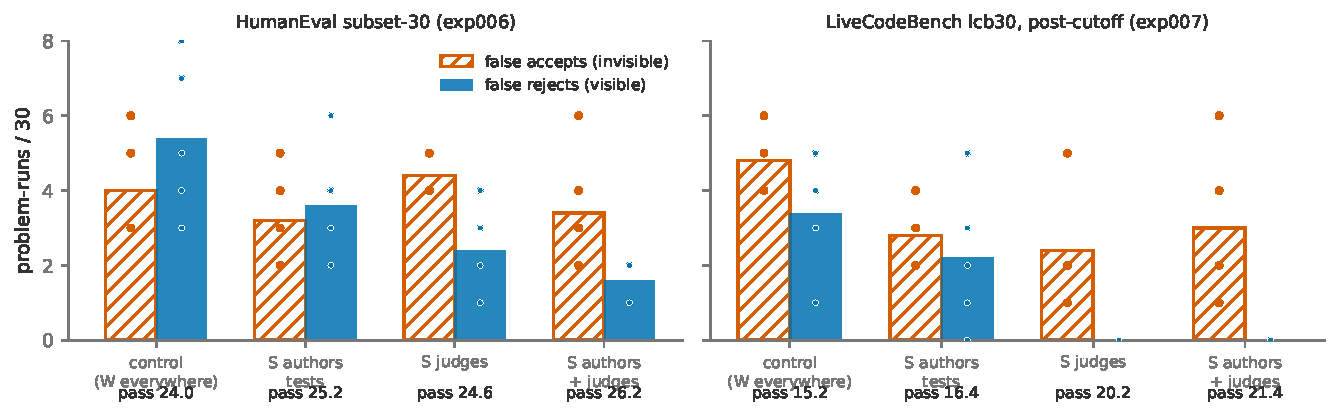
\includegraphics[width=\linewidth]{figures/fig2_asym.pdf}
\caption{False accepts (hatched) and false rejects (solid) per cell; bars are means, dots the
five runs; oracle pass means beneath each cell. The asymmetry is the finding: false accepts
are flat everywhere, while the strong-judge cells drive false rejects toward zero and (right
panel) lift pass rates.}
\label{fig:asym}
\end{figure}

\subsection{RQ2: frontier models in the verification roles}
\label{sec:results-asym}

\paragraph{The false-accept count does not meet the decision bar in any case.} There are eight cells, two
benchmarks, and three ways to place a frontier model in verification: in none does the
false-accept contrast reach the decision bar. On HumanEval, the counts do not even shift in the
expected direction with the judge ($4.0 \to 3.2/4.4/3.4$, all $p{=}1.0$; the frontier-judge cell
is higher than control); on LiveCodeBench, they trend downward ($4.8 \to 2.8/2.4/3.0$) but no
contrast is significant ($p \in [0.125, 0.375]$), and we note the direction: at $N{=}5$, an effect
of this size cannot be separated from run noise. This was the pre-registered confirmatory
prediction (H-B2), and it holds: the probability that a claimed success is wrong remains
substantial, $2.4$--$4.4$ per run, regardless of who grades. The remaining false accepts are not
due to weak-model carelessness that a stronger verifier would catch; they are the structural blind
spot built into the loop.
% trace: exp006 ANALYSIS.md contrasts; exp007 ANALYSIS.md contrasts (FA rows)

\paragraph{The null result holds for two more frontier verifiers.} A skeptic might accept the null for one
just-released model of untested verification ability but still suspect it is unique to that model.
We pre-registered and repeated the entire asymmetry design with two more frontier verifiers, chosen
for the opposite trait: Gemini-2.5-Pro, the top-ranked code judge on an execution-grounded judge
benchmark~\cite{jiang2025codejudgebench}, and Claude-4.5-Sonnet, the latest release of the
second-ranked Sonnet line. With the weak generator fixed and only the strong role changed, across
both benchmarks and all twelve strong cells, not a single false-accept contrast meets the decision
bar (Table~\ref{tab:verifiers}, Figure~\ref{fig:verifiers}): two of the strongest reported code
judges leave the false-accept count where the weak model left it, while false rejects again drop
under the strong judge (both LiveCodeBench judge cells and both HumanEval judge cells show
reductions). The soundness null now holds across all three frontier verifiers we test---GPT-5.6
Terra, Gemini-2.5-Pro, and Claude-4.5-Sonnet, covering OpenAI, Anthropic, and Google, and unknown,
first-, and second-ranked judging lines. This claim is made specifically for the verifiers and
benchmarks we measured, not for all models.
% trace: exp011 {he,lcb}_{claude,gemini}/ANALYSIS.md (FA and FR rows)

\begin{table}[t]
\centering
\small
\caption{False accepts per 30-problem run (mean, $N{=}5$) under three frontier verifiers, each
swapped into the test-author (\emph{S tests}), judge (\emph{S judge}), or both roles against the
fixed weak generator. For every verifier, on both benchmarks, no strong-cell contrast clears the
decision bar---the false-accept count is statistically indistinguishable from the all-weak control.
GPT-5.6 Terra is exp006/exp007; Gemini-2.5-Pro and Claude-4.5-Sonnet are the pre-registered exp011
replication (Sec.~\ref{sec:results-asym}). HumanEval is scored with HumanEval\texttt{+}.}
\label{tab:verifiers}
\begin{tabular}{lrrrr}
\toprule
Frontier verifier S & control & S tests & S judge & S both \\
\midrule
\multicolumn{5}{l}{\emph{HumanEval}\texttt{+}} \\
\quad GPT-5.6 Terra     & $4.0$ & $3.2$ & $4.4$ & $3.4$ \\
\quad Gemini-2.5-Pro    & $4.8$ & $3.2$ & $4.0$ & $4.8$ \\
\quad Claude-4.5-Sonnet & $3.8$ & $2.8$ & $3.4$ & $4.2$ \\
\midrule
\multicolumn{5}{l}{\emph{LiveCodeBench} (hidden, post-cutoff oracle)} \\
\quad GPT-5.6 Terra     & $4.8$ & $2.8$ & $2.4$ & $3.0$ \\
\quad Gemini-2.5-Pro    & $3.8$ & $1.8$ & $3.4$ & $2.6$ \\
\quad Claude-4.5-Sonnet & $3.6$ & $2.0$ & $3.4$ & $3.6$ \\
\bottomrule
\end{tabular}
\end{table}

\begin{figure}[t]
\centering
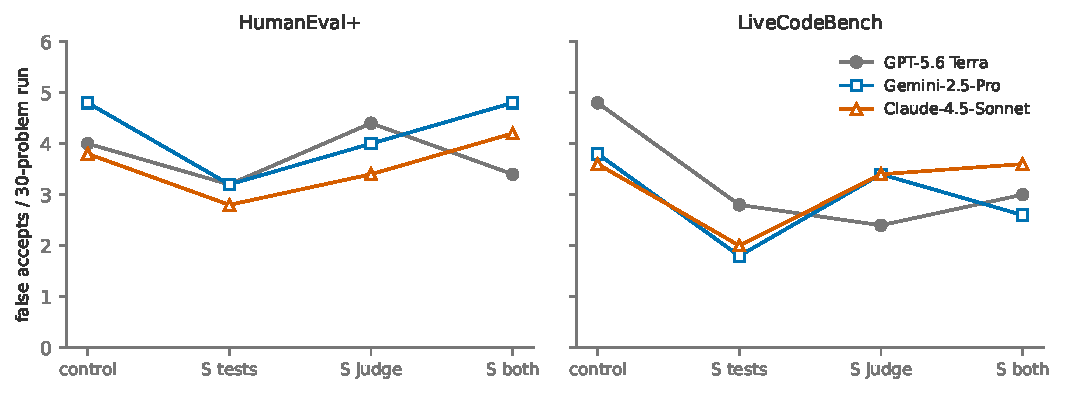
\includegraphics[width=0.82\linewidth]{figures/fig5_verifiers.pdf}
\caption{False accepts stay flat across the role assignments, for every verifier. Each line is one
frontier verifier swapped into the verification roles; none falls with verifier strength on either
benchmark (same data as Table~\ref{tab:verifiers}).}
\label{fig:verifiers}
\end{figure}

\paragraph{False rejects disappear when the frontier judge is used.} On LiveCodeBench, both
frontier-judge cells show \emph{zero} false rejects in all ten runs (control: $3.4$); on
HumanEval, they fall from $5.4$ to $2.4$ (judge) and $1.6$ (both), and each difference
exceeds the minimum effect size. When the loop wrongly rejects correct code, the frontier
judge nearly eliminates this problem.
% trace: exp006/exp007 ANALYSIS.md (FR rows)

\paragraph{For out-of-distribution cases, the frontier judge raises the pass rate. These are
the only significant signals in the matrix.} On LiveCodeBench, oracle passes rise from $15.2$
to $20.2$ (judge; $\Delta{+}5.0$, $p{=}.0312$) and $21.4$ (both; $\Delta{+}6.2$, $p{=}.0156$),
passing the decision threshold. On HumanEval, the same cells increase by $+0.6$ and $+2.2$,
which is within the margin of error: near the weak model's in-distribution ceiling, feedback has
little left to recover, but on new problems, there is much more room to improve.
% trace: exp007 ANALYSIS.md contrasts (pass rows)

\paragraph{A frontier test author does not change the pass rate.} The cell practitioners might
focus on---a frontier model writing the tests while the weak model codes against them---leaves the
oracle pass rate unchanged from control on both benchmarks ($+1.2$ on each, within noise), with FA
and FR also within noise. This is registered as an open directional hypothesis
(H-B3); the result is null. One descriptive detail: on LiveCodeBench, its \emph{total} verdict
error drops past that composite's effect-size threshold ($8.2 \to 5.0$), with both error
directions trending downward, a smaller verdict-side benefit but no generation benefit, which
matches the mechanism account below.
% trace: exp006/exp007 ANALYSIS.md (strong_testgen rows)

\subsection{RQ3: the improvement flows through feedback}
\label{sec:results-mech}

The pipeline's telemetry reveals the mechanism. Canonical (anchored) tests stay constant at
$75$ per run in every LCB cell; the anchoring requirement is fully met. What changes is the number of
tests the judge calls for beyond those: control suites have about $76$ tests per run; the
frontier judge's \texttt{ADD:} directives raise suites to $182$--$194$, and cycle completions
go from about $17/30$ to $23$--$24/30$, while completed cycles remain correct at a similar rate.
The judge's effect is passed through the retry loop's feedback channel, with richer tests
guiding the weak generator toward correct solutions, not through its accept verdicts, whose error
rate (the false accepts) never meets the threshold in any cell. The strong test author also writes
larger suites ($140$ per run), but only once, with no iterative pressure on the generator: the
pass rate stays the same, and only the composite verdict error improves.
% trace: exp007 ANALYSIS.md (tests_per_run/canonical rows); launch logs (TDD success counts)

\subsection{RQ4: the gap widens at application scale}
\label{sec:results-scale}

On RGRBench, the gap is not just a small-problem artifact; it is larger. In the control
cell, $65$ of $261$ valid runs end in a self-claimed success, and $41.5\%$ of those claims fail
the hand-verified oracle ($95\%$ Wilson CI $[30.4, 53.7]$); the strong-judge cell claims $50$
successes out of $251$ valid runs at a statistically similar $42.0\%$ ($[29.4, 55.8]$). The
design's $267$ runs per cell reduce to $261$ and $251$ valid runs because the pre-registered
protocol excludes evaluations with no usable oracle verdict: in $21$ of the $22$ excluded runs,
the oracle collected zero tests because the generated adapter failed to import the candidate
package at collection time, and one control run failed due to a harness environment error. This is
about double the $18\%$/$29\%$ seen in the algorithmic benchmarks, and even the lower confidence
bound ($30\%$) is higher than their point estimates. Figure~\ref{fig:misalignment} shows one
of these false accepts on a fully specified package. RGRBench evaluates a candidate using a
generated \emph{adapter} that re-exposes it under the oracle's expected import names, statically
constrained so it cannot bring any of its own behavior, allowing us to directly limit the
adapter's contribution to these numbers; an automated calibration sets it at $0.000$
(Sec.~\ref{sec:threats}). Three pre-registered properties clarify the situation
(Table~\ref{tab:scale}).
% trace: exp010 results/ANALYSIS.md (control/strong_judge H-D1); calibration/calibration.json

\begin{figure}[t]
\centering
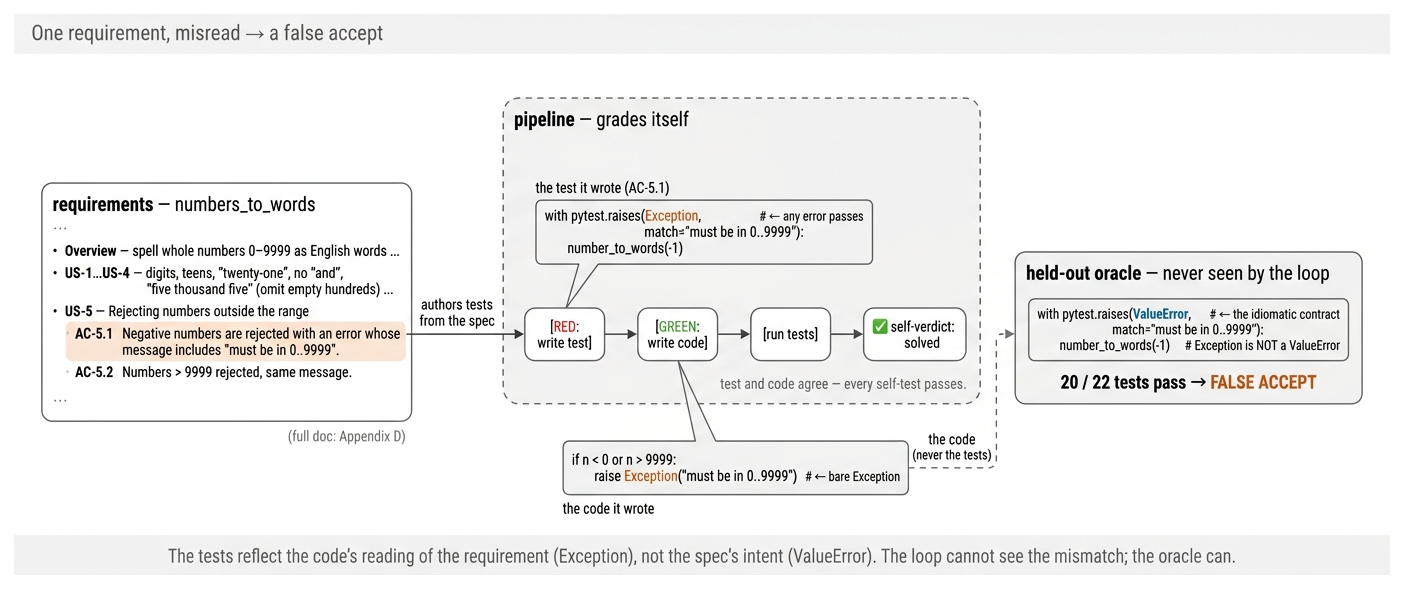
\includegraphics[width=\linewidth]{figures/fig6_misalignment.png}
\caption{A false accept on a fully specified requirement (RGRBench's \texttt{numbers\_to\_words}).
AC-5.1 pins the error \emph{message} but not its Python \emph{type}; the pipeline's own test
accepts any \texttt{Exception}, the code raises one, and the two agree---so the loop reports
success. The held-out oracle encodes the idiomatic contract (\texttt{ValueError}), which a bare
\texttt{Exception} does not satisfy, and two of the twenty-two tests fail. The tests inherited the
code's misreading, so nothing inside the loop could catch it. Full requirements, tests, code, and
oracle in App.~\ref{app:telephone}.}
\label{fig:misalignment}
\end{figure}

\begin{table}[t]
\centering
\caption{RGRBench (application scale): the self-verification confusion matrix and the
false-accept analyses, over $N{=}3$ runs of $89$ packages ($534$ runs). Control = weak model
everywhere; strong-judge = frontier model in all judge roles. TA/FA/FR/TR are counts over
valid runs (accept/reject $\times$ oracle pass/fail); oracle-passing solutions $=$ TA${+}$FR.
Conditional FA is FA as a fraction of claimed successes (TA${+}$FA); tier and attempt rows
restrict that quantity to each subset. Brackets are $95\%$ Wilson intervals.}
\label{tab:scale}
\small
\begin{tabular}{lcc}
\toprule
 & control & strong-judge \\
\midrule
valid runs                           & 261 & 251 \\
true accepts (TA)                    & 38  & 29  \\
false accepts (FA)                   & 27  & 21  \\
false rejects (FR, H-D3)             & 14  & 0   \\
true rejects (TR)                    & 182 & 201 \\
oracle-passing solutions (TA${+}$FR) & 52  & 29  \\
\midrule
claimed successes (TA${+}$FA)        & 65 & 50 \\
conditional FA (H-D1) & 0.415 [0.304, 0.537] & 0.420 [0.294, 0.558] \\
\quad beginner tier (H-D4) & 0.31 & 0.38 \\
\quad intermediate tier & 0.54 & 0.50 \\
\quad advanced tier & 0.86 & 0.75 \\
first- / multi-attempt FA (H-D2) & 0.35 / 0.64 & 0.34 / 0.67 \\
\bottomrule
\end{tabular}
\end{table}

\paragraph{The gap grows with task complexity.} Conditional false accepts rise steadily
across the three difficulty tiers (Figure~\ref{fig:complexity}): $31\% \to 54\% \to 86\%$ in the
control cell, and $38\% \to 50\% \to 75\%$ under the strong judge. On the hardest tier, six out of
seven claimed successes are wrong. This is a scaling dimension that single-function benchmarks
cannot show. The gap is not a fixed cost; it grows with the complexity that leads one to use an
agent in the first place.
% trace: exp010 results/ANALYSIS.md (H-D4 rows)

\begin{figure}[t]
\centering
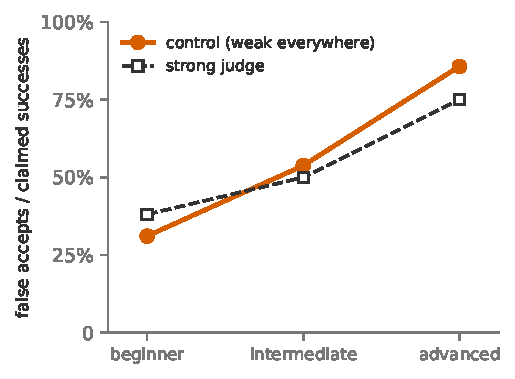
\includegraphics[width=0.52\linewidth]{figures/fig3_complexity.pdf}
\caption{Conditional false accepts rise monotonically with difficulty tier on RGRBench, in both
cells (H-D4). This is a scaling axis single-function benchmarks cannot exhibit, and the strong
judge does not flatten it.}
\label{fig:complexity}
\end{figure}

\paragraph{Refinement makes the problem worse.} Claims that the pipeline reaches only after
retrying are false about twice as often as first-attempt claims: $64\%$ versus $35\%$ (control)
and $67\%$ versus $34\%$ (strong judge). The loop's own iteration, presented as self-correction,
leads to more confident errors, independently repeating the ``refinement worsens
overfitting'' effect reported on SWE-bench~\cite{ahmed2025overfitting}.
% trace: exp010 results/ANALYSIS.md (H-D2 rows)

\paragraph{Soundness invariance, a third time.} The frontier judge leaves the false-accept
rate statistically unchanged ($41.5\% \to 42.0\%$) while eliminating false rejects completely
($14 \to 0$), repeating the soundness invariance of the two algorithmic experiments
at application scale on a third independent instrument (the false-reject collapse, however,
reads differently here---see the next paragraph). Across HumanEval\texttt{+}
($18\%$), a post-cutoff LiveCodeBench window ($29\%$), and RGRBench ($42\%$), and alongside
the external SWE-bench overfitting measurements
($\sim$$20$--$33\%$~\cite{ahmed2025overfitting,yu2026sweabs}), the false-accept gap of a
self-testing loop appears under every oracle we test (Figure~\ref{fig:convergence}) and is not
reduced by verifier strength. We report this as a recurring pattern under three oracles and one
pipeline family; the threshold sweep below shows it is a tradeoff a stronger verifier never
improves, not a constant of nature.
% trace: exp010 results/ANALYSIS.md (H-D1/H-D3); exp006/exp007 ANALYSIS.md (conditional FA)

\paragraph{At application scale the judge acts as a gate, not a coach.} When seen as a
full confusion matrix (Table~\ref{tab:scale}), the false-reject collapse does not have the same
completeness meaning that it does on algorithmic benchmarks. The frontier judge \emph{lowers}
the pipeline's correct output: oracle-passing solutions drop from $52$ to $29$ and true accepts
from $38$ to $29$.\footnote{Restricting to the $249$ (package, run) pairs valid in both cells gives
the same picture: oracle passes $49 \to 29$, and of the packages one cell solves and the other does
not, $24$ are lost by the strong judge against $4$ gained; the conditional false-accept rate moves
$36.8\% \to 40.8\%$.} The RED gate causes this, not repair---the frontier judge rejects
the self-authored test suite on $189$ of $251$ runs, which are then abandoned before any code is
written ($62$ reach GREEN, compared to $258$ under the weak judge). The survivors are individually
stronger (oracle-correct $46.8\%$ versus $20.2\%$), but there are far too few to make up the
difference. As a result, false rejects disappear not because correct solutions are recovered but
because they are never created at all---the mass shifts from FR to TR. At application scale the
frontier judge does not achieve greater soundness ($41.5\% \to 42.0\%$) or net completeness
($38 \to 29$ true accepts); the coaching effect we see on single-function problems
(Sec.~\ref{sec:discussion}) does not appear here. Even the false-accept rate itself is not fixed:
it is determined by the RED acceptance threshold, which is examined next.
% trace: exp010 results/ (result.json: self_verdict x oracle.pass_fraction; red_attempts/green_attempts)

\paragraph{The false-accept rate depends on the threshold; it is not a fixed value.} The $42\%$
figure above is just one operating point. A pre-registered sweep of the RED acceptance
threshold $\tau$ on the strong-judge cell (exp013; $\tau \in \{0.40, 0.50, 0.55, 0.70, 0.85\}$)
moves the rate between $33\%$ and $68\%$ (Table~\ref{tab:tausweep}). Loosening the gate
($\tau{:}\,0.70 \to 0.40$) increases the rate from $42\%$ to $67.6\%$ [$51.5, 80.4$] as more claims
are accepted; tightening the threshold reduces output but does not lower the rate below about
$42\%$. The matched point is straightforward: at $\tau{=}0.50$ ($N{=}3$), the frontier judge
accepts as much as the weak control ($31.5\%$ versus $24.9\%$) at a false-accept rate that is not
lower---$47.5\%$ [$36.9, 58.3$] compared to $41.5\%$ [$30.4, 53.7$], higher in point estimate but
with overlapping intervals. The situation only gets worse as more are admitted: at
$\tau{=}0.40$ ($43.0\%$ acceptance), the rate is $67.6\%$ [$51.5, 80.4$]. The $41.5\% \to 42.0\%$
agreement at the shared $\tau{=}0.70$ came from the frontier judge accepting fewer claims, not from
any improvement in soundness due to its strength. Making the verifier stronger does not reduce the
false-accept rate: at matched throughput it stays the same, and it rises as more are admitted.
The difference is a throughput--soundness tradeoff within the loop, and a stronger judge does not
shift it toward soundness.
% trace: experiments/exp013_tau_sweep/results/ANALYSIS.md; PRE_REGISTRATION.md (H1 refuted; H2; H3)

\begin{table}[t]
\centering
\caption{RED-threshold sweep on the strong-judge RGRBench cell (exp013, pre-registered). The
matched-acceptance point $\tau{=}0.50$ is confirmatory ($N{=}3$, $89$ packages); the other new
$\tau$ points are $N{=}1$; $\tau{=}0.70$ is the exp010 anchor ($N{=}3$). The weak-judge control is
shown for the matched comparison. Loosening the gate raises both acceptance and the false-accept
rate. Brackets are $95\%$ Wilson intervals.}
\label{tab:tausweep}
\small
\begin{tabular}{lccc}
\toprule
cell & accept\% & FA\% [$95\%$] & RED-gate\% \\
\midrule
control (weak), $\tau{=}0.70$      & $24.9$ & $41.5$ [$30.4, 53.7$] & $1.1$  \\
strong, $\tau{=}0.85$              & $7.4$  & $33.3$ [$9.7, 70.0$]  & $91.4$ \\
strong, $\tau{=}0.70$              & $19.9$ & $42.0$ [$29.4, 55.8$] & $75.3$ \\
strong, $\tau{=}0.55$              & $20.0$ & $52.9$ [$31.0, 73.8$] & $72.9$ \\
strong, $\tau{=}0.50$ ($N{=}3$)    & $31.5$ & $47.5$ [$36.9, 58.3$] & $62.6$ \\
strong, $\tau{=}0.40$              & $43.0$ & $67.6$ [$51.5, 80.4$] & $47.7$ \\
\bottomrule
\end{tabular}
\end{table}

\begin{figure}[t]
\centering
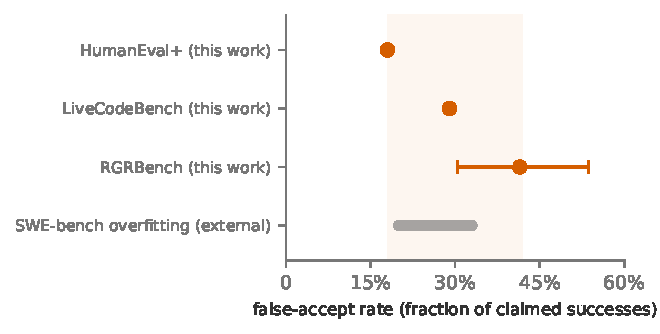
\includegraphics[width=0.66\linewidth]{figures/fig4_convergence.pdf}
\caption{The false-accept gap of a self-testing loop appears under every oracle we test and is not
reduced by verifier strength.
Three independent instruments (HumanEval\texttt{+}, a post-cutoff LiveCodeBench window, and
RGRBench with its $95\%$ Wilson interval) land in the same band as the external SWE-bench
overfitting literature~\cite{ahmed2025overfitting,yu2026sweabs}. The RGRBench point is one
threshold on the tradeoff of Table~\ref{tab:tausweep}, not a fixed constant.}
\label{fig:convergence}
\end{figure}

\section{Discussion}
\label{sec:discussion}

\paragraph{Completeness improves; soundness does not.} The two types of error respond to
verifier strength in opposite ways, and this split is meaningful. False rejects are errors the loop
can \emph{detect}: a test fails, the cycle retries, and feedback accumulates. A stronger judge uses
that visibility to drive repair, and on new problems it eliminates this error class entirely,
with zero false rejects in all ten frontier-judge runs. False accepts, on the other hand, are
failures the loop \emph{cannot represent}: tests and code both pass, every internal signal is green,
and there is nothing left for any judge, no matter how capable, to inspect. The judge evaluates the
tests based on its interpretation of the specification; when the test author's misunderstanding is
plausible, the judge simply makes that reading \emph{more} internally consistent. It does not
check whether the reading matches the meaning of the specification. Adding model strength
inside the loop improves completeness because those failures are visible within the loop; it cannot
improve soundness, since soundness failures, by design, are not visible.

\paragraph{The judge serves as a coach, not a gatekeeper.} The largest effect in either
matrix---the five-to-six-problem pass-rate increase on unseen cases---is not a verification effect at
all. It is the frontier judge \emph{teaching} the weak pipeline through required tests and directive
feedback, which is shown in the tripled suite sizes and the restored cycle completions. This
changes the production intuition that led to the experiments: asymmetric deployments (with a cheap
generator and a frontier model in the loop) are valuable, and our data suggests that the value is
concentrated in the judge's role rather than that of the test author. However, this coaching effect
depends on scale: on RGRBench, the same frontier judge instead acts as a strict gate, abandoning
most packages at RED and \emph{reducing} net correct output instead of increasing it
(Sec.~\ref{sec:results-scale}), so the asymmetric deployment is efficient for single-function
problems but not clearly so at application scale. Still, the underlying mechanism is generation
quality, not verdict quality. The verdicts that matter for trust---``this is correct, ship it''---are
just as unreliable as before.

\paragraph{Implication for builders.} A self-testing pipeline's accept verdict does not
show correctness at any verifier strength that the loop can purchase, and the
improvement from stronger models only makes the verdicts more frequent (more cycles
finish) without making them more reliable. A pipeline that completes more cycles and
self-accepts at the same false-accept rate will just ship \emph{more} incorrect code, but with
greater confidence. The calibration channel must come from outside the loop: held-out test
suites, differential testing against independent implementations, or tracking verdicts versus
true outcomes on problems with known answers. No component inside the loop can provide that
calibration.

\paragraph{Why the strong test author disappoints.} The null result on frontier-authored tests
is the study's most unexpected finding. One way to read this: test quality is determined by
iteration, not by who writes the tests. A suite written once, no matter how skillfully, does
not push back against a weak generator's misreadings, while an adversarial reviewer of the weak
model's own suites forces the specification to be re-examined with every retry. This is an
exploratory interpretation; the pre-registered fact is simply the null.

\paragraph{The gap is a validation failure, born at comprehension.} Every intervention we test
happens after the moment when a natural-language specification is turned into a test suite, and
none of them changes the false-accept rate, because the misalignment is set at that first moment,
not later. In requirements engineering terms, the loop performs \emph{verification} perfectly
(the code is built correctly, according to its tests) but never performs \emph{validation} (the
tests themselves are correct, faithful to the intent)~\cite{boehm1984vv}. Seen this way, the
soundness-invariance result is less surprising and almost a tautology: no amount of verification
strength can close a validation gap, because they answer different questions. This failure is not
new to LLMs. It is the classic requirements ``telephone game,'' where a specification, filtered
through each reader's domain assumptions, leads to systems built correctly but for the wrong
intent. Waterfall methods took months or years to reveal these errors, and agile only sped up the
process when an external oracle (a customer, a failing production case) could reveal the
misunderstanding. A self-testing agent removes that oracle and repeats the same misunderstanding
at inference speed. The pattern holds even when the input is already structured. On RGRBench, the
pipeline receives a user-story requirements document with explicit acceptance criteria, not just a
bare prompt, and the false-accept rate is still $42\%$ (Figure~\ref{fig:misalignment} traces one
such false accept end to end). Structure at the story level does not remove the interpretive
freedom of the natural-language-to-test step where the gap starts.

\paragraph{Attacking the initial conditions.} If the gap is created at comprehension, the lever
our experiments never move is the \emph{input} to test authoring. Breaking down and clarifying a
specification into refined stories and acceptance criteria precise enough to read almost like
pseudo-code for the tests would reduce the interpretive distance the RED author must cross,
lowering the gap's initial size instead of trying to catch it later, which is what our
strong-judge and strong-author cells try and fail to do. We did not test this, and one caution
follows from the reframing above: a refinement stage that generates its own acceptance criteria
self-consistently just moves the comprehension step; it does not remove it. Such a front-end is
most likely to help when the refined criteria are validated against intent from outside the loop:
a human sign-off on the acceptance criteria, in the spirit of TiCoder's interactive test
validation~\cite{fakhoury2024ticoder} but applied to the requirements layer. Building and
measuring such a front-end on RGRBench is the constructive next step this diagnosis suggests.

\section{Threats to Validity}
\label{sec:threats}

\paragraph{Construct.} The gap is defined in relation to an oracle; if the oracle is weak, it
understates the gap, and any flaws in the oracle itself will carry over. We measure against
three oracles at increasing distances (visible-adjacent, strong, hidden), and the effect remains
under all three. Self-verdicts are execution outcomes captured by the harness, not just model
claims. On RGRBench, two more safeguards are in place. The oracle's blind spots are measured and
bounded, not just assumed (mutation kill rate $0.981$, each surviving mutant is individually
classified), so the error in the held-out suite is a directly measured value. Also, since
RGRBench uses a generated adapter for grading, a mis-mapped adapter could theoretically increase
false accepts; to check this, an automated calibration distorts each package's known-correct
reference solution into a foreign API (using a behavior-preserving AST transform) and regrades it
through a blind, model-written adapter, so any failure here is purely due to the adapter. Behavior
preservation is checked for each package before it is counted, and the measured adapter-caused
false-accept rate is $0.000$ across all tiers (13 usable packages, including the most difficult).
The application-scale gap is not just a technical artifact.
% trace: experiments/exp010_flagship/calibrate_adapter.py, calibration/calibration.json;
% trace: rgrbench instrument/mutation_scores.json, equivalent_mutants.md

\paragraph{Application-scale selection.} The two RGRBench cells differ only by the judge model,
yet that difference changes \emph{which} packages get a verdict: at the pre-registered threshold
$\tau{=}0.70$, the frontier judge rejects the self-authored tests on $189$ out of $251$ runs
(Sec.~\ref{sec:results-scale}), so its reported successes come from a much smaller, judge-selected
survivor set than the control's. Two results follow. The cross-cell false-accept rate is then
compared across these shifted selection regimes; we report the matched-set rate on packages valid
in both cells as the direct comparison, and it does not move more than the raw rate. The
pre-registered $\tau$-sweep and matched-acceptance design (exp013, Sec.~\ref{sec:results-scale})
address the calibration question directly: the RED-gate abandonment does track $\tau$ but remains
well above the weak judge's rate even at the most permissive threshold, so it is both
threshold-driven and intrinsic; and at matched acceptance ($\tau{=}0.50$, $N{=}3$) its
false-accept rate is not lower than the control's---higher in point estimate but overlapping, and
clearly worse only as it admits more---so the shared-$\tau$ agreement reflected its stricter
selection, not a gain in soundness. The application-scale results still depend on a single
frontier judge (GPT-5.6 Terra); whether the threshold tradeoff and completeness reversal
apply to other frontier judges at this scale is not yet tested, and three of the four new
$\tau$ points still have $N{=}1$.

\paragraph{Internal.} We study a single pipeline. Its full instrument (engine, prompts, and the
defect register from a line-by-line review) is included with the artifact, and every reported
number is from that instrument.

\paragraph{External.} There are now three benchmarks and three frontier verifiers: two
single-function algorithmic benchmarks and RGRBench's $89$ multi-concern packages, with the strong
role filled in turn by GPT-5.6 Terra, Gemini-2.5-Pro, and Claude-4.5-Sonnet, each from a different
provider (Table~\ref{tab:verifiers}). Two robustness checks were pre-registered: moving to
application-scale, test-first-built corpora with hand-verified oracles made the finding stronger
(Sec.~\ref{sec:results-scale}), and verifier replication reproduced the soundness null on every
benchmark. What remains is generator diversity---the generator is \emph{intentionally} kept at one
weak model to isolate the verifier's effect---and a public leaderboard over many generator/verifier
systems on RGRBench, left as future work for the released benchmark. The verifiers' training cutoffs
differ, and some exposure to the LCB window is possible for the later two; the design is robust in
the important direction, since memorization of solutions by the judge could only \emph{lower} false
accepts, and across all three verifiers, the rates did not change. The pass-rate increase, though,
could in principle be inflated by exposure; its mechanism (test volume, feedback, completions) is
measured, not just assumed. Only one pipeline is studied; the protocol can be used elsewhere, but
the constants are specific.

\paragraph{Conclusion validity.} Per-problem outcomes vary between identical runs; we
pre-registered practical minimums along with significance tests, confirmed that these minimums were
conservative compared to observed control spreads, and treat differences below the threshold as
noise, regardless of $p$-value. With $N{=}5$ runs per cell, the power is limited: effects smaller
than these minimums would not be detected, which is why the invariance claim is stated as ``within
pre-registered noise,'' not as proof of no effect.

\paragraph{Execution safety.} The pipeline runs model-generated tests and code as standard
subprocesses, each in a temporary per-run working directory with a fixed interpreter and
\texttt{PYTHONPATH} limited to that directory, under wall-clock timeouts ($30$\,s per test run,
$120$\,s per oracle run). This limits runaway execution but is not a hardened sandbox: there is
no container, no memory or CPU limit, and no network isolation. Running untrusted model output
at larger scale should add OS-level isolation.

\paragraph{Anchoring.} The RED prompts anchor one test per canonical example
(App.~\ref{app:prompts}); we tested this across four variants (both sides, generator-only,
judge-only, neither) on three generator models, all included in the artifact. Across these
variants, the overall pass and self-verdict rates change only slightly. The case studies in
App.~\ref{app:cases} show why anchoring cannot close the gap: it ensures the specification's
worked examples are covered, but covering examples is not the same as covering the specification,
and every false accept we examined passes the anchored examples but fails on other inputs. A
false-accept-instrumented anchoring ablation across models is left as future work for the released
benchmark.

\section{Conclusion}
\label{sec:conclusion}

A pipeline that writes its own tests is also grading itself, and nothing inside the loop is
assigned to grade the grader. We defined the verification gap to make that missing function
measurable, measured it on three benchmarks (one with problems the generator had never seen and
whose tests were never in any prompt, and one built at application scale with hand-checked,
error-barred oracles), then paid for the obvious fix: a frontier model in the verification roles.
The report card is wrong about roughly one claimed success in four, and it stays wrong under a
frontier test author, a frontier judge, and both together---and under all three frontier verifiers
we tried, across three providers. What the frontier judge provides is worth having: false rejects
disappear, and on new problems its feedback raises true pass rates by a third. Still, it is a
better coach, not a better gatekeeper, and every improvement comes through the feedback channel
while the accept verdicts remain blind. Verification strength inside a self-testing loop buys
completeness, not soundness. And the blind spot is not just a small-problem issue. On RGRBench's
application-scale, multi-concern packages, the report card is wrong about two claims in five, worse
where the tasks are harder and even worse after the loop's own retries: the same failure, just
larger where the programs look more like those agents ship. For builders, the implication is
architectural. The accept verdict of a self-testing agent is not evidence at any internal verifier
strength, and calibration must come from outside the loop: held-out oracles, differential checks,
verdict accounting, or, upstream, a requirement grounded in intent before it is ever turned into a
test, since the gap is created in that translation and not in the grading that follows. No
assignment of models to the roles inside the loop removes it.

\bibliographystyle{plainnat}
\bibliography{refs}

\appendix

\section{Defect register of the studied pipeline (summary)}
\label{app:register}

A line-by-line review of the pipeline surfaced 15 harness defects (H-1--H-15: import-time
side effects, environment-dependent tool invocation, missing response logging, list-content
crashes on 2026 models, usage-logger stacking) and nine behavioral defects
(Table~\ref{tab:register}). All harness defects and behavioral defects B-1--B-8 are fixed in
the study instrument; B-10's underlying mechanism was later removed outright, so the failure
analyst no longer produces code at all and nothing the judge writes can ship. The
prompt templates were separately rewritten after review (Sec.~\ref{sec:prompts}). Identifiers are stable against the
repository's full register, which includes locations, failure scenarios, and dispositions;
that register never assigned the identifier B-9, so the nine behavioral defects carry the
identifiers B-1--B-8 and B-10, and Table~\ref{tab:register} has no B-9 row by construction.
% trace: src/vgap/pipeline/REVIEW.md (B-9 was never assigned; IDs kept stable)

\begin{table}[h]
\centering
\caption{Behavioral defects found during review; disposition in the study instrument.}
\label{tab:register}
\small
\begin{tabular}{lll}
\toprule
ID & Finding & Disposition \\
\midrule
B-1 & Template render errors silently become empty prompts upstream & fixed \\
B-2 & Hanging generated test aborts the whole problem run & fixed \\
B-3 & Judge pass/fail verdicts via substring scan of the entire response & fixed \\
B-4 & First-match score regex; ``Score: 85'' normalizes to a perfect 1.0 & fixed \\
B-5 & GREEN judge verdict threshold hardcoded at 0.7, ignoring configuration & fixed \\
B-6 & Two result classes with different validation semantics across judges & fixed \\
B-7 & Latent \texttt{NameError} in the RED retry fallback (unreachable) & fixed \\
B-8 & GREEN's execution gate tests one file; VERIFY tests the whole suite & fixed \\
B-10 & Judge-corrected code never ships; travels only as prompt text & mechanism removed \\
\bottomrule
\end{tabular}
\end{table}

\section{Prompt skeletons}
\label{app:prompts}

Abbreviated structure of the two RED-phase templates (the GREEN pair follows the same
pattern; full templates in the artifact). Anchoring blocks are marked in the source and
removed mechanically to create ablation variants.

\paragraph{RED generator (test author).}
\begin{small}
\begin{verbatim}
You are writing the test suite for a Python function BEFORE any
implementation exists (TDD, RED phase). Your tests are the only
specification the implementer will see [...]
## Task                     <- title, description, signatures
## Specification details    <- full problem statement
## Scenarios to cover       <- worked examples from the spec
[ANCHOR] ## MANDATORY: Canonical Examples from Specification
  For EVERY example: one test named test_canonical_example_N with
  the EXACT inputs and EXACT expected output + derivation comment.
## Rules  1. only specified behavior ... 5. plain pytest
## Reviewer feedback on your previous suite   <- retry only
## Output: one fenced ```python block, nothing else
\end{verbatim}
\end{small}

\paragraph{RED judge (test reviewer).}
\begin{small}
\begin{verbatim}
Judge one thing only: does this suite faithfully verify the
specification? [...]
[ANCHOR] ## Check 0 - MANDATORY Canonical Example Coverage
  any missing/altered example => Final score: 0.00
## Checks  1. fidelity (recompute every expected value)
           2. no invented constraints  3. coverage  4. sanity
## Scoring: deduction schedule (0.30/0.30/0.20/0.10, floor 0)
## Output: findings; ADD:/REMOVE:/FIX: directives (apply-verbatim);
           last line exactly `Final score: <x.xx>`
\end{verbatim}
\end{small}

\section{False-accept case studies}
\label{app:cases}

Every false accept follows the same pattern: the self-authored suite anchors itself to the
specification's worked examples (the anchoring block of App.~\ref{app:prompts} enforces one
\texttt{test\_canonical\_example} per example), the implementation passes these, and both miss
a behavior that the held-out oracle checks. Three HumanEval false accepts make this pattern
specific: two from the all-weak control and one from the cell with a frontier judge, each accepted
with a top GREEN-judge score. Code and tests are copied exactly from the committed run logs.

\paragraph{HumanEval/32 (\texttt{find\_zero}, control cell).} The spec requests a root of an
arbitrary even-degree polynomial. The self-suite tests only the two docstring examples
(\texttt{find\_zero([1,2])} $\rightarrow -0.5$, \texttt{find\_zero([-6,11,-6,1])} $\rightarrow
1.0$). The implementation uses Newton's method starting from \texttt{x=0.0} for $100$
iterations. Newton-from-zero converges on both example polynomials, so the suite passes, but this
is not a general root-finder: when the iteration stalls (\texttt{dfx==0}, and it breaks) or
diverges, it returns a non-root. HumanEval\texttt{+}'s extra polynomials cause exactly
this, and the oracle rejects. The tests only confirm the two points the code was tailored for, not
the full specification.

\paragraph{HumanEval/74 (\texttt{total\_match}, control cell).} The spec returns the list with
the smaller total character count, \emph{and returns the first list if the totals are equal}.
The implementation handles the tie incorrectly: \texttt{if total1 < total2: return lst1} else
\texttt{return lst2}, so equal totals default to \texttt{lst2}. None of the five generated
example tests presents a clear tie---the only equal-total case is \texttt{([],[])}, where
both answers are \texttt{[]}, so the tie branch is never tested. HumanEval\texttt{+} includes
an equal-total pair with different contents; the code returns the second list where the spec
requires the first, and the oracle rejects.

\paragraph{HumanEval/153 (\texttt{Strongest\_Extension}, frontier-judge cell).} Strength is
calculated as (uppercase count) minus (lowercase count); the strongest extension is the one with
the highest value, with ties going to the earliest occurrence. The implementation sets the running
maximum to \texttt{0} at the start and only updates it when \texttt{strength > strongest\_strength}.
This means if every extension has a strength of zero or less, and the strongest is not the first
one, the loop never updates and it ends up returning \texttt{extensions[0]}. The two generated
tests do not trigger this scenario---example~1 is all-negative, but its first element is already
the strongest, so the bug is hidden. As a result, the suite passes, and the frontier judge gave it
a score of $1.0$. HumanEval\texttt{+} provides an all-negative case where the maximum is not the
first, and in that case, the oracle rejects it.

\paragraph{At application scale.} The same signature appears again in RGRBench. The
\texttt{strong\_judge} run on \texttt{numbers\_to\_words} certifies itself, but the held-out oracle
only passes $20$ out of its $22$ tests; App.~\ref{app:telephone} repeats this false accept
completely. The per-package artifacts (including self-authored tests, the generated package, and
the oracle's result) are committed for all $534$ runs.

\section{An RGRBench false accept in full: \texttt{numbers\_to\_words}}
\label{app:telephone}

The false accept of Figure~\ref{fig:misalignment}, laid out end to end. The pipeline sees only
the requirements below; from them it authors its tests and its implementation, and reports success
once the implementation passes those tests. The held-out oracle is applied afterward and never
enters the loop. The implementation is correct on every spelling rule; the single defect is the
exception \emph{type} on the range check---which the requirement leaves implicit (it fixes the
message, not the type), the pipeline's own test does not specify (it accepts any
\texttt{Exception}), and the oracle does (it demands \texttt{ValueError}).

\paragraph{Requirements given to the pipeline.} User-story narratives are omitted; the acceptance
criteria are verbatim.
\begin{small}
\begin{verbatim}
# Spelling numbers as English words

## Overview
A number-spelling service turns any whole number from 0 through
9999 into its English words, following everyday conventions:
hyphenated compounds for twenty-one through ninety-nine, no "and"
between parts, and plain spaces between the thousands, hundreds,
and remainder portions.

### US-1: Spelling numbers up to twenty
- AC-1.1: Zero is spelled "zero", and single digits use their
  names, such as "five" and "eight".
- AC-1.2: Ten is spelled "ten", and the teens are single
  unhyphenated words, such as "thirteen" and "nineteen".

### US-2: Spelling two-digit numbers
- AC-2.1: Round tens are single words with no hyphen, such as
  "twenty" and "ninety".
- AC-2.2: Other two-digit numbers are hyphenated tens-units
  compounds: 21 is "twenty-one", 77 is "seventy-seven", and 99
  is "ninety-nine".

### US-3: Spelling hundreds
- AC-3.1: 100 is "one hundred"; the leading "one" is always kept.
- AC-3.2: A hundreds part is followed by the spelled remainder
  separated by a space: 303 is "three hundred three", 555 is
  "five hundred fifty-five", and 115 is "one hundred fifteen".
- AC-3.3: The word "and" never joins the hundreds to the
  remainder.

### US-4: Spelling thousands
- AC-4.1: 1000 is "one thousand" with the leading "one" kept,
  and round thousands follow the same pattern, such as "two
  thousand".
- AC-4.2: The thousands part is followed by the spelled
  remainder: 2400 is "two thousand four hundred", 3466 is "three
  thousand four hundred sixty-six", and an empty hundreds part is
  simply omitted, so 5005 is "five thousand five".
- AC-4.3: The largest supported number, 9999, is "nine thousand
  nine hundred ninety-nine".

### US-5: Rejecting numbers outside the range
- AC-5.1: Negative numbers are rejected with an error whose
  message includes "must be in 0..9999".
- AC-5.2: Numbers greater than 9999 are rejected with the same
  error message wording.
\end{verbatim}
\end{small}

\paragraph{Tests the pipeline authored (range check).} It also wrote a passing test for every
spelling rule; the two range checks are the ones that decide this case. Each asks only for a
generic \texttt{Exception}.
\begin{small}
\begin{verbatim}
def test_reject_negative_numbers():
    with pytest.raises(Exception, match=r"must be in 0\.\.9999"):
        number_to_words(-1)                        # AC-5.1

def test_reject_numbers_greater_than_[...]ninety_nine():
    with pytest.raises(Exception, match=r"must be in 0\.\.9999"):
        number_to_words(10000)                     # AC-5.2
\end{verbatim}
\end{small}

\paragraph{The generated implementation.} Digit tables and the remainder-spelling branch (both
correct) are omitted with \texttt{...} and \texttt{[...]}; all other lines are verbatim. The range
check raises a bare \texttt{Exception}.
\begin{small}
\begin{verbatim}
def number_to_words(n):
    if n < 0 or n > 9999:
        raise Exception("must be in 0..9999")
    if n == 0:
        return "zero"
    units = ["", "one", "two", ...]      # digit tables abbreviated
    teens = ["ten", "eleven", "twelve", ...]
    tens = ["", "", "twenty", "thirty", ...]
    thousands = n // 1000
    hundreds = (n % 1000) // 100
    remainder = n % 100
    words = []
    if thousands:
        words.append(units[thousands] + " thousand")
    if hundreds:
        words.append(units[hundreds] + " hundred")
    if remainder:
        [...]  # spell the 0..99 remainder, hyphenating 21..99
    return " ".join(words)
\end{verbatim}
\end{small}

\paragraph{The held-out oracle (applied after the loop).} The other twenty tests cover the
spelling rules and all pass; the two range checks require \texttt{ValueError}, which a bare
\texttt{Exception} is not, so running the full oracle against the implementation gives $20$ of
$22$.
\begin{small}
\begin{verbatim}
def test_negative_numbers_are_rejected() -> None:
    with pytest.raises(ValueError, match="must be in 0..9999"):
        number_to_words(-1)

def test_numbers_above_9999_are_rejected() -> None:
    with pytest.raises(ValueError, match="must be in 0..9999"):
        number_to_words(10000)
\end{verbatim}
\end{small}

\end{document}
